%!TEX root = ../main.tex

\newpage
\section*{Supplementary}

  \renewcommand{\thefigure}{S\arabic{figure}}
  \setcounter{figure}{0}

  \renewcommand{\thetable}{S\arabic{table}}
  \setcounter{table}{0}

  \begin{table}[H]
\centering
\small
\begin{tabular}{|c|c|c|c|c|}
\hline
\textbf{Step}                         & \textbf{Task}                   & \textbf{Module}                                   & \textbf{Parameter}           & \textbf{Value}   \\ \hline
\multirow{14}{*}{Sequence Processing} & \multirow{6}{*}{Demultiplexing} & \multirow{3}{*}{demultiplexing\_illumina\_single} & barcode\_column              & barcode-sequence \\
                                      &                                 &                                                   & rev\_comp\_barcodes          & false            \\
                                      &                                 &                                                   & rev\_comp\_mapping\_barcodes & false            \\ \cline{3-5}
                                      &                                 & \multirow{3}{*}{demultiplexing\_illumina\_paired} & barcode\_column              & barcode-sequence \\
                                      &                                 &                                                   & rev\_comp\_barcodes          & false            \\
                                      &                                 &                                                   & rev\_comp\_mapping\_barcodes & false            \\ \cline{2-5}
                                      & \multirow{8}{*}{Trimming}       & export\_visualization\_single                     & seq\_samplesize              & 10000            \\ \cline{3-5}
                                      &                                 & export\_visualization\_paired                     & seq\_samplesize              & 10000            \\ \cline{3-5}
                                      &                                 & \multirow{3}{*}{trimming\_single}                 & ncpus                        & 1                \\
                                      &                                 &                                                   & max\_ee                      & 2                \\
                                      &                                 &                                                   & trunc\_q                     & 2                \\ \cline{3-5}
                                      &                                 & \multirow{3}{*}{trimming\_paired}                 & ncpus                        & 1                \\
                                      &                                 &                                                   & max\_ee                      & 2                \\
                                      &                                 &                                                   & trunc\_q                     & 2                \\ \hline
\end{tabular}
\caption{The default parameters used in the Sequence Processing step of the \ac{micone} pipeline}
\label{tab:sp_parameters}
\end{table}

\begin{table}[H]
\centering
\small
\begin{tabular}{lllll}
\hline
\textbf{Step}                             & \textbf{Task}                                            & \textbf{Tool}                          & \textbf{Parameter}                     & \textbf{Value}                                                                                           \\ \hline
\multirow{17}{*}{Sequence Processing}     & \multirow{4}{*}{Bootstrap}                               & \multirow{3}{*}{resample}              & bootstraps                             & 1000                                                                                                     \\
                                          &                                                          &                                        & ncpus                                  & 1                                                                                                        \\
                                          &                                                          &                                        & filter\_flag                           & True                                                                                                     \\
                                          &                                                          & pvalue                                 & ncpus                                  & 1                                                                                                        \\ \cline{2-5}
                                          & \multirow{12}{*}{Correlation}                            & \multirow{2}{*}{sparcc}                & iterations                             & 50                                                                                                       \\
                                          &                                                          &                                        & ncpus                                  & 1                                                                                                        \\
                                          &                                                          & pearson                                & -                                      & -                                                                                                        \\
                                          &                                                          & spearman                               & -                                      & -                                                                                                        \\
                                          &                                                          & \multirow{5}{*}{spieceasi}             & method                                 & mb                                                                                                       \\
                                          &                                                          &                                        & ncpus                                  & 1                                                                                                        \\
                                          &                                                          &                                        & nreps                                  & 50                                                                                                       \\
                                          &                                                          &                                        & nlambda                                & 20                                                                                                       \\
                                          &                                                          &                                        & lambda\_min\_ratio                     & 1e-2                                                                                                     \\
                                          &                                                          & \multirow{2}{*}{mldm}                  & z\_mean                                & 1                                                                                                        \\
                                          &                                                          &                                        & max\_iteration                         & 1500                                                                                                     \\
                                          &                                                          & magma                                  & -                                      & -                                                                                                        \\ \cline{2-5}
                                          & Network                                                  & make\_network                          & -                                      & -                                                                                                        \\ \hline
\end{tabular}
\caption{The default parameters used in the various tools of the pipeline}
\label{tab:all_parameters}
\end{table}

\begin{table}[H]
\centering
\small
\begin{tabular}{lllll}
\hline
\textbf{Step}                             & \textbf{Task}                                            & \textbf{Tool}                          & \textbf{Parameter}                     & \textbf{Value}                                                                                           \\ \hline
\multirow{29}{*}{Denosing and Clustering} & \multicolumn{1}{c}{\multirow{9}{*}{Sequence Processing}} & \multirow{2}{*}{join\_reads}           & min\_overlap                           & 6                                                                                                        \\
                                          & \multicolumn{1}{c}{}                                     &                                        & perc\_max\_diff                        & 8                                                                                                        \\
                                          & \multicolumn{1}{c}{}                                     & \multirow{2}{*}{demultiplex\_illumina} & rev\_comp\_barcodes                    & False                                                                                                    \\
                                          & \multicolumn{1}{c}{}                                     &                                        & rev\_comp\_mapping\_barcodes           & False                                                                                                    \\
                                          & \multicolumn{1}{c}{}                                     & demultiplex\_454                       & -                                      & -                                                                                                        \\
                                          & \multicolumn{1}{c}{}                                     & \multirow{4}{*}{trim\_filter\_fixed}   & seq\_sample\_size                      & 10,000                                                                                                   \\
                                          & \multicolumn{1}{c}{}                                     &                                        & ncpus                                  & 1                                                                                                        \\
                                          & \multicolumn{1}{c}{}                                     &                                        & trunc\_q                               & 2                                                                                                        \\
                                          & \multicolumn{1}{c}{}                                     &                                        & max\_ee                                & 2                                                                                                        \\ \cline{2-5}
                                          & \multirow{3}{*}{Chimera Checking}                        & uchime                                 & -                                      & -                                                                                                        \\
                                          &                                                          & \multirow{2}{*}{remove\_bimera}        & ncpus                                  & 1                                                                                                        \\
                                          &                                                          &                                        & chimera\_method                        & consensus                                                                                                \\ \cline{2-5}
                                          & \multirow{17}{*}{Denoise Cluster}                        & \multirow{3}{*}{de\_novo}              & enable\_rev\_strand\_match             & True                                                                                                     \\
                                          &                                                          &                                        & suppress\_de\_novo\_chimera\_detection & True                                                                                                     \\
                                          &                                                          &                                        & ncpus                                  & 1                                                                                                        \\
                                          &                                                          & \multirow{4}{*}{closed\_reference}     & enable\_rev\_strand\_match             & True                                                                                                     \\
                                          &                                                          &                                        & suppress\_de\_novo\_chimera\_detection & True                                                                                                     \\
                                          &                                                          &                                        & ncpus                                  & 1                                                                                                        \\
                                          &                                                          &                                        & reference\_sequences                   & 97\_otus.fasta                                                                                           \\
                                          &                                                          & \multirow{5}{*}{open\_reference}       & enable\_rev\_strand\_match             & True                                                                                                     \\
                                          &                                                          &                                        & suppress\_de\_novo\_chimera\_detection & True                                                                                                     \\
                                          &                                                          &                                        & ncpus                                  & 1                                                                                                        \\
                                          &                                                          &                                        & reference\_sequences                   & 97\_otus.fasta                                                                                           \\
                                          &                                                          &                                        & picking\_method                        & uclust                                                                                                   \\
                                          &                                                          & \multirow{2}{*}{dada2}                 & ncpus                                  & 1                                                                                                        \\
                                          &                                                          &                                        & big\_data                              & FALSE                                                                                                    \\
                                          &                                                          & \multirow{3}{*}{deblur}                & ncpus                                  & 1                                                                                                        \\
                                          &                                                          &                                        & mind\_reads                            & 2                                                                                                        \\
                                          &                                                          &                                        & min\_size                              & 2                                                                                                        \\ \hline
\end{tabular}
\caption{The default parameters used in the various tools of the pipeline}
\label{tab:all_parameters}
\end{table}


\begin{table}[H]
\centering
\small
\begin{tabular}{lllll}
\hline
\textbf{Step}                             & \textbf{Task}                                            & \textbf{Tool}                          & \textbf{Parameter}                     & \textbf{Value}                                                                                           \\ \hline
\multirow{7}{*}{Taxonomy Assignment}      & \multirow{7}{*}{Assign}                                  & \multirow{3}{*}{naive\_bayes}          & confidence                             & 0.7                                                                                                      \\
                                          &                                                          &                                        & mem\_per\_core                         & 8G                                                                                                       \\
                                          &                                                          &                                        & ncpus                                  & 1                                                                                                        \\
                                          &                                                          & \multirow{4}{*}{blast}                 & max\_accepts                           & 10                                                                                                       \\
                                          &                                                          &                                        & perc\_identity                         & 0.8                                                                                                      \\
                                          &                                                          &                                        & evalue                                 & 0.001                                                                                                    \\
                                          &                                                          &                                        & min\_consensus                         & 0.51                                                                                                     \\ \hline
\end{tabular}
\caption{The default parameters used in the various tools of the pipeline}
\label{tab:all_parameters}
\end{table}


\begin{table}[H]
\centering
\small
\begin{tabular}{lllll}
\hline
\textbf{Step}                             & \textbf{Task}                                            & \textbf{Tool}                          & \textbf{Parameter}                     & \textbf{Value}                                                                                           \\ \hline
\multirow{12}{*}{OTU/ESV Processing}      & \multirow{5}{*}{Filter}                                  & \multirow{3}{*}{abundance}             & count\_thres                           & 500                                                                                                      \\
                                          &                                                          &                                        & prevalence\_thres                      & 0.05                                                                                                     \\
                                          &                                                          &                                        & abundance\_thres                       & 0.01                                                                                                     \\
                                          &                                                          & group                                  & tax\_levels                            & \begin{tabular}[c]{@{}l@{}}{[}'Phylum', 'Class', 'Order',\\ 'Family', 'Genus', 'Species'{]}\end{tabular} \\
                                          &                                                          & partition                              & -                                      & -                                                                                                        \\ \cline{2-5}
                                          & \multirow{6}{*}{Transform}                               & \multirow{6}{*}{normalize}             & count\_thres                           & 500                                                                                                      \\
                                          &                                                          &                                        & axis                                   & sample                                                                                                   \\
                                          &                                                          &                                        & prevalence\_thres                      & 0.05                                                                                                     \\
                                          &                                                          &                                        & abundace\_thres                        & 0.01                                                                                                     \\
                                          &                                                          &                                        & rm\_sparse\_obs                        & True                                                                                                     \\
                                          &                                                          &                                        & rm\_sparse\_samples                    & True                                                                                                     \\ \cline{2-5}
                                          & Export                                                   & biom2tsv                               & -                                      & -                                                                                                        \\ \hline
\end{tabular}
\caption{The default parameters used in the various tools of the pipeline}
\label{tab:all_parameters}
\end{table}


\begin{table}[H]
\centering
\small
\begin{tabular}{lllll}
\hline
\textbf{Step}                             & \textbf{Task}                                            & \textbf{Tool}                          & \textbf{Parameter}                     & \textbf{Value}                                                                                           \\ \hline
\multirow{17}{*}{Network Inference}       & \multirow{4}{*}{Bootstrap}                               & \multirow{3}{*}{resample}              & bootstraps                             & 1000                                                                                                     \\
                                          &                                                          &                                        & ncpus                                  & 1                                                                                                        \\
                                          &                                                          &                                        & filter\_flag                           & True                                                                                                     \\
                                          &                                                          & pvalue                                 & ncpus                                  & 1                                                                                                        \\ \cline{2-5}
                                          & \multirow{12}{*}{Correlation}                            & \multirow{2}{*}{sparcc}                & iterations                             & 50                                                                                                       \\
                                          &                                                          &                                        & ncpus                                  & 1                                                                                                        \\
                                          &                                                          & pearson                                & -                                      & -                                                                                                        \\
                                          &                                                          & spearman                               & -                                      & -                                                                                                        \\
                                          &                                                          & \multirow{5}{*}{spieceasi}             & method                                 & mb                                                                                                       \\
                                          &                                                          &                                        & ncpus                                  & 1                                                                                                        \\
                                          &                                                          &                                        & nreps                                  & 50                                                                                                       \\
                                          &                                                          &                                        & nlambda                                & 20                                                                                                       \\
                                          &                                                          &                                        & lambda\_min\_ratio                     & 1e-2                                                                                                     \\
                                          &                                                          & \multirow{2}{*}{mldm}                  & z\_mean                                & 1                                                                                                        \\
                                          &                                                          &                                        & max\_iteration                         & 1500                                                                                                     \\
                                          &                                                          & magma                                  & -                                      & -                                                                                                        \\ \cline{2-5}
                                          & Network                                                  & make\_network                          & -                                      & -                                                                                                        \\ \hline
\end{tabular}
\caption{The default parameters used in the various tools of the pipeline}
\label{tab:all_parameters}
\end{table}

  
  \subsection{Configuration used for MiCoNE runs}
  
  \subsection{Generation of sequence data}
  
  \subsubsection{Mock sequence data}
  Mock 4: A mock community composed of 21 bacterial strains represented in equal abundances in two replicate samples, and the same strains represented in uneven abundances in two replicate samples. These are the same community members present in mock-3 and mock-5, which consists of the same mock community samples analyzed on separate Illumina sequencing runs. This was generated by Dr. Dirk Gevers at Broad Institute in 2012. Previously called dataset-3 in [Bokulich et al. 2013](https://dx.doi.org/10.1038/nmeth.2276) and dataset B4 in [Bokulich et al. 2015](https://dx.doi.org/10.7287/peerj.preprints.934v2).
  
  Mock 12: Composed of 27 bacterial strains amplified with 515f/806r primers. Intended to include more closely related taxa than the other mock communities, the members of which were chosen in part for their well-separated 16S rRNA gene sequences. These strains are all distinguishable over the sequenced region of the 16S rRNA gene, but some pairs of strains differ by as little as one nucleotide. Generated by Benjamin Callahan at Stanford University in 2015. Known as "Extreme" dataset in the original publication, doi:10.1038/nmeth.3869.
  
  Mock 16: Mock community generated by Melanie Schirmer at University of Glasgow in 2015. Composed of even amounts of purified genomic DNA from 49 bacteria and 10 archaea. Known as dataset 35 in the original publication, doi:10.1093/nar/gku1341.
  
  \subsubsection{Synthetic sequence data}
  - We first create a sequence pool for various samples. This will have mutated (2\% mutation rate) reference sequences at abundances that are close to real abundances
  - We then use `art_illumina` with 1x fold_coverage to generate fastq read files for each sample.

    We created reference sequences that are 1/10th or 1/100th such that we have repeating sequences. Eg. If we have 3500 total reads, and 90\% are from same taxonomy, we have 32 or 315 reads of this sequence then we can fix `-f` as 3500/multiplier. To get multiplier we  could look at low abundant sequence and how much do we need to have atleast one of these sequences. OR should I just have fold coverage of 1x and 3500 references? Make 2\% of the positions in each sequence randomly mutate to create nucleotide diversity [source](https://www.ncbi.nlm.nih.gov/pmc/articles/PMC5967554/)

  \subsection{Generation of synthetic interaction data}
  Figures describing the original OTU tables or the interactions used to generate the community. Also include the seed and scripts for reproducing the networks.

  \begin{figure}[h]
  \centering
  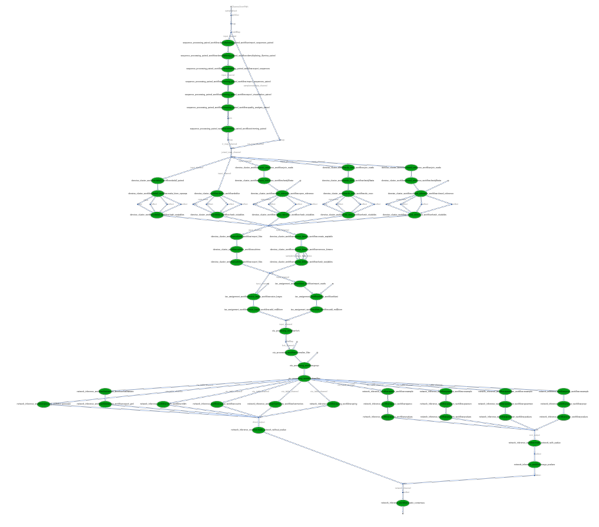
\includegraphics[width=\linewidth]{figureS1.pdf}
  \caption{
    \textbf{Comparison of various denoising and clustering algorithms used in the pipeline}.
    (A, B) Correlation of the abundances of the taxa that are in common between the count matrices created by two different methods.
    (A) The worst correlation (least similar methods) is between open-reference and dada2.
    (B) The best correlation (most similar methods) is between open-reference and denovo.
    (C) A heatmap showing the $\mathrm{R}^2$ of all pairwise comparisons of the methods.
  }
  \label{fig:figureS1}
\end{figure}

  \begin{figure}[h]
    \centering
    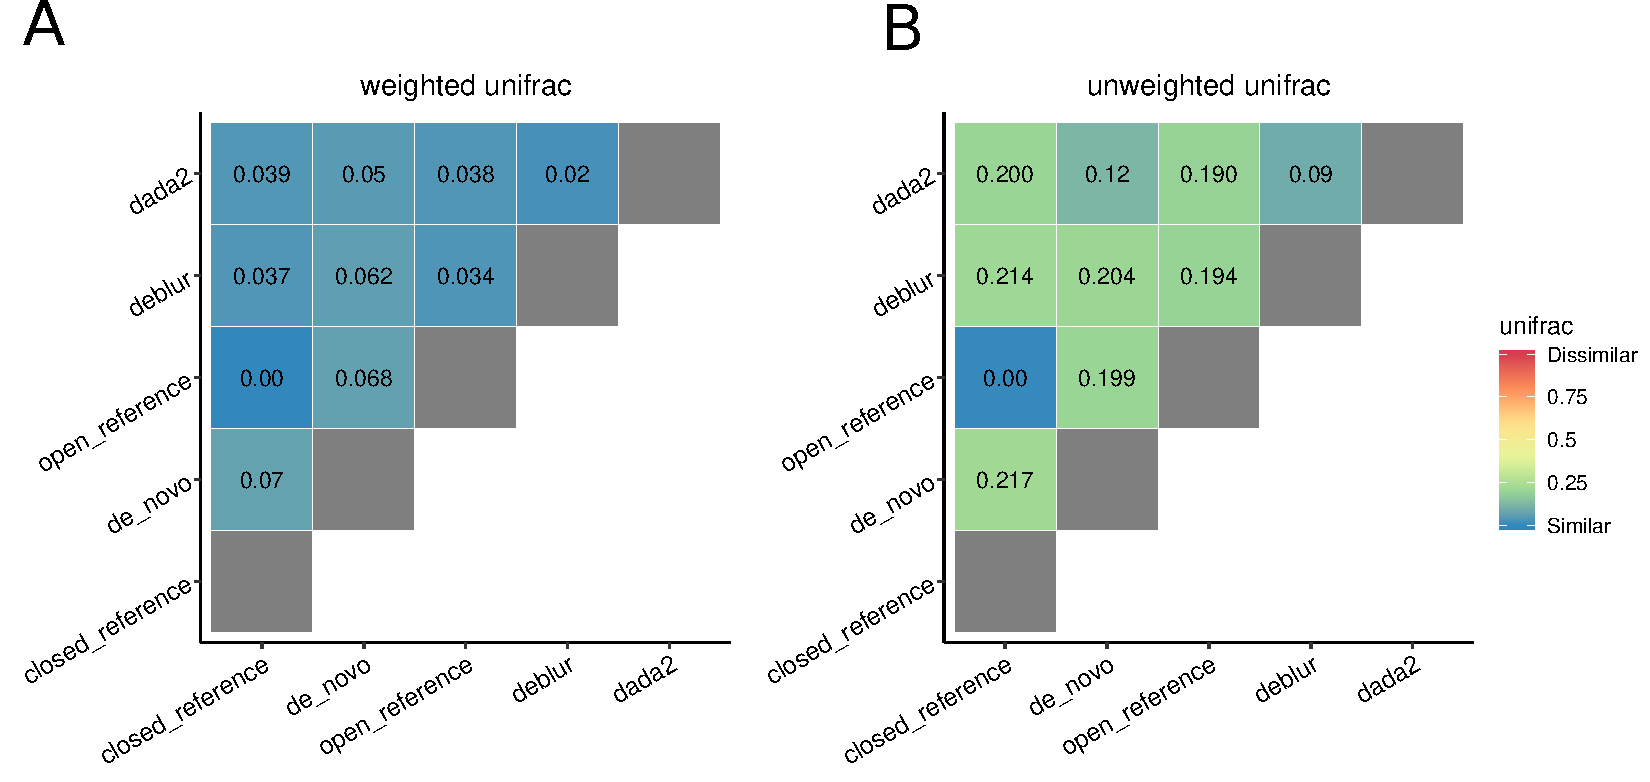
\includegraphics[width=\linewidth]{figureS2.pdf}
    \caption{
      \textbf{Heatmaps showing the weighted and unweighted unifrac distances for the hard palate dataset analysis}.
      (A) weighted unifrac distances and (B) unweighted unifrac distances between the representative sequences generated by different denoising and clustering algorithms.
      These results are in agreement with the stool microbiome dataset.
    }
    \label{fig:figureS2}
  \end{figure}

  \begin{figure}[h]
    \centering
    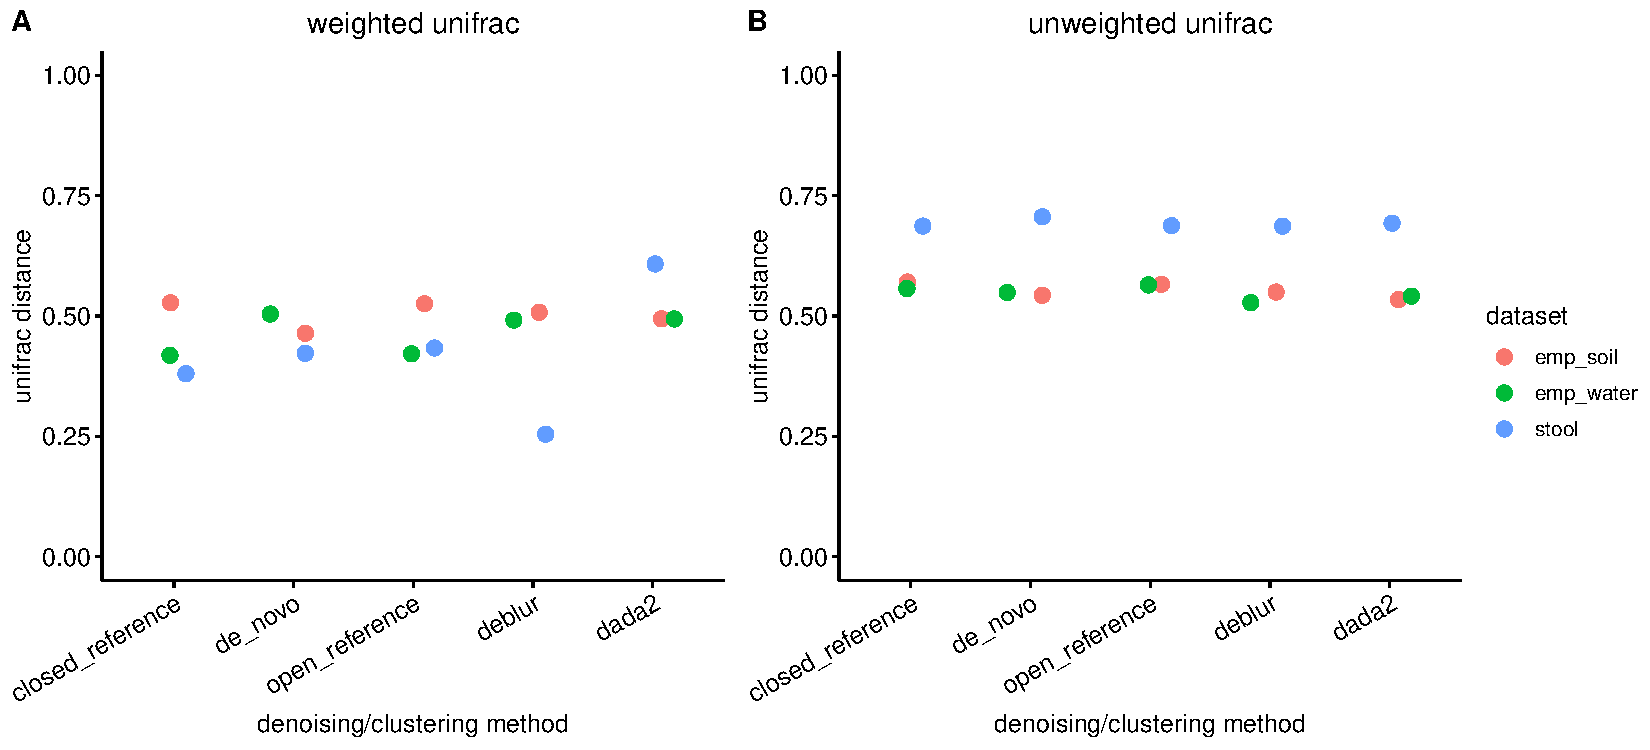
\includegraphics[width=\linewidth]{figureS3.pdf}
    \caption{
      \textbf{The distributions of the average weighted UniFrac distance between the expected sequence profile and the calculated sequence profile in the synthetic datasets}.
      We observe no significant difference between the various methods on the synthetic datasets used for this study.
    }
    \label{fig:figureS3}
  \end{figure}

%   \begin{figure}[h]
%     \centering
%     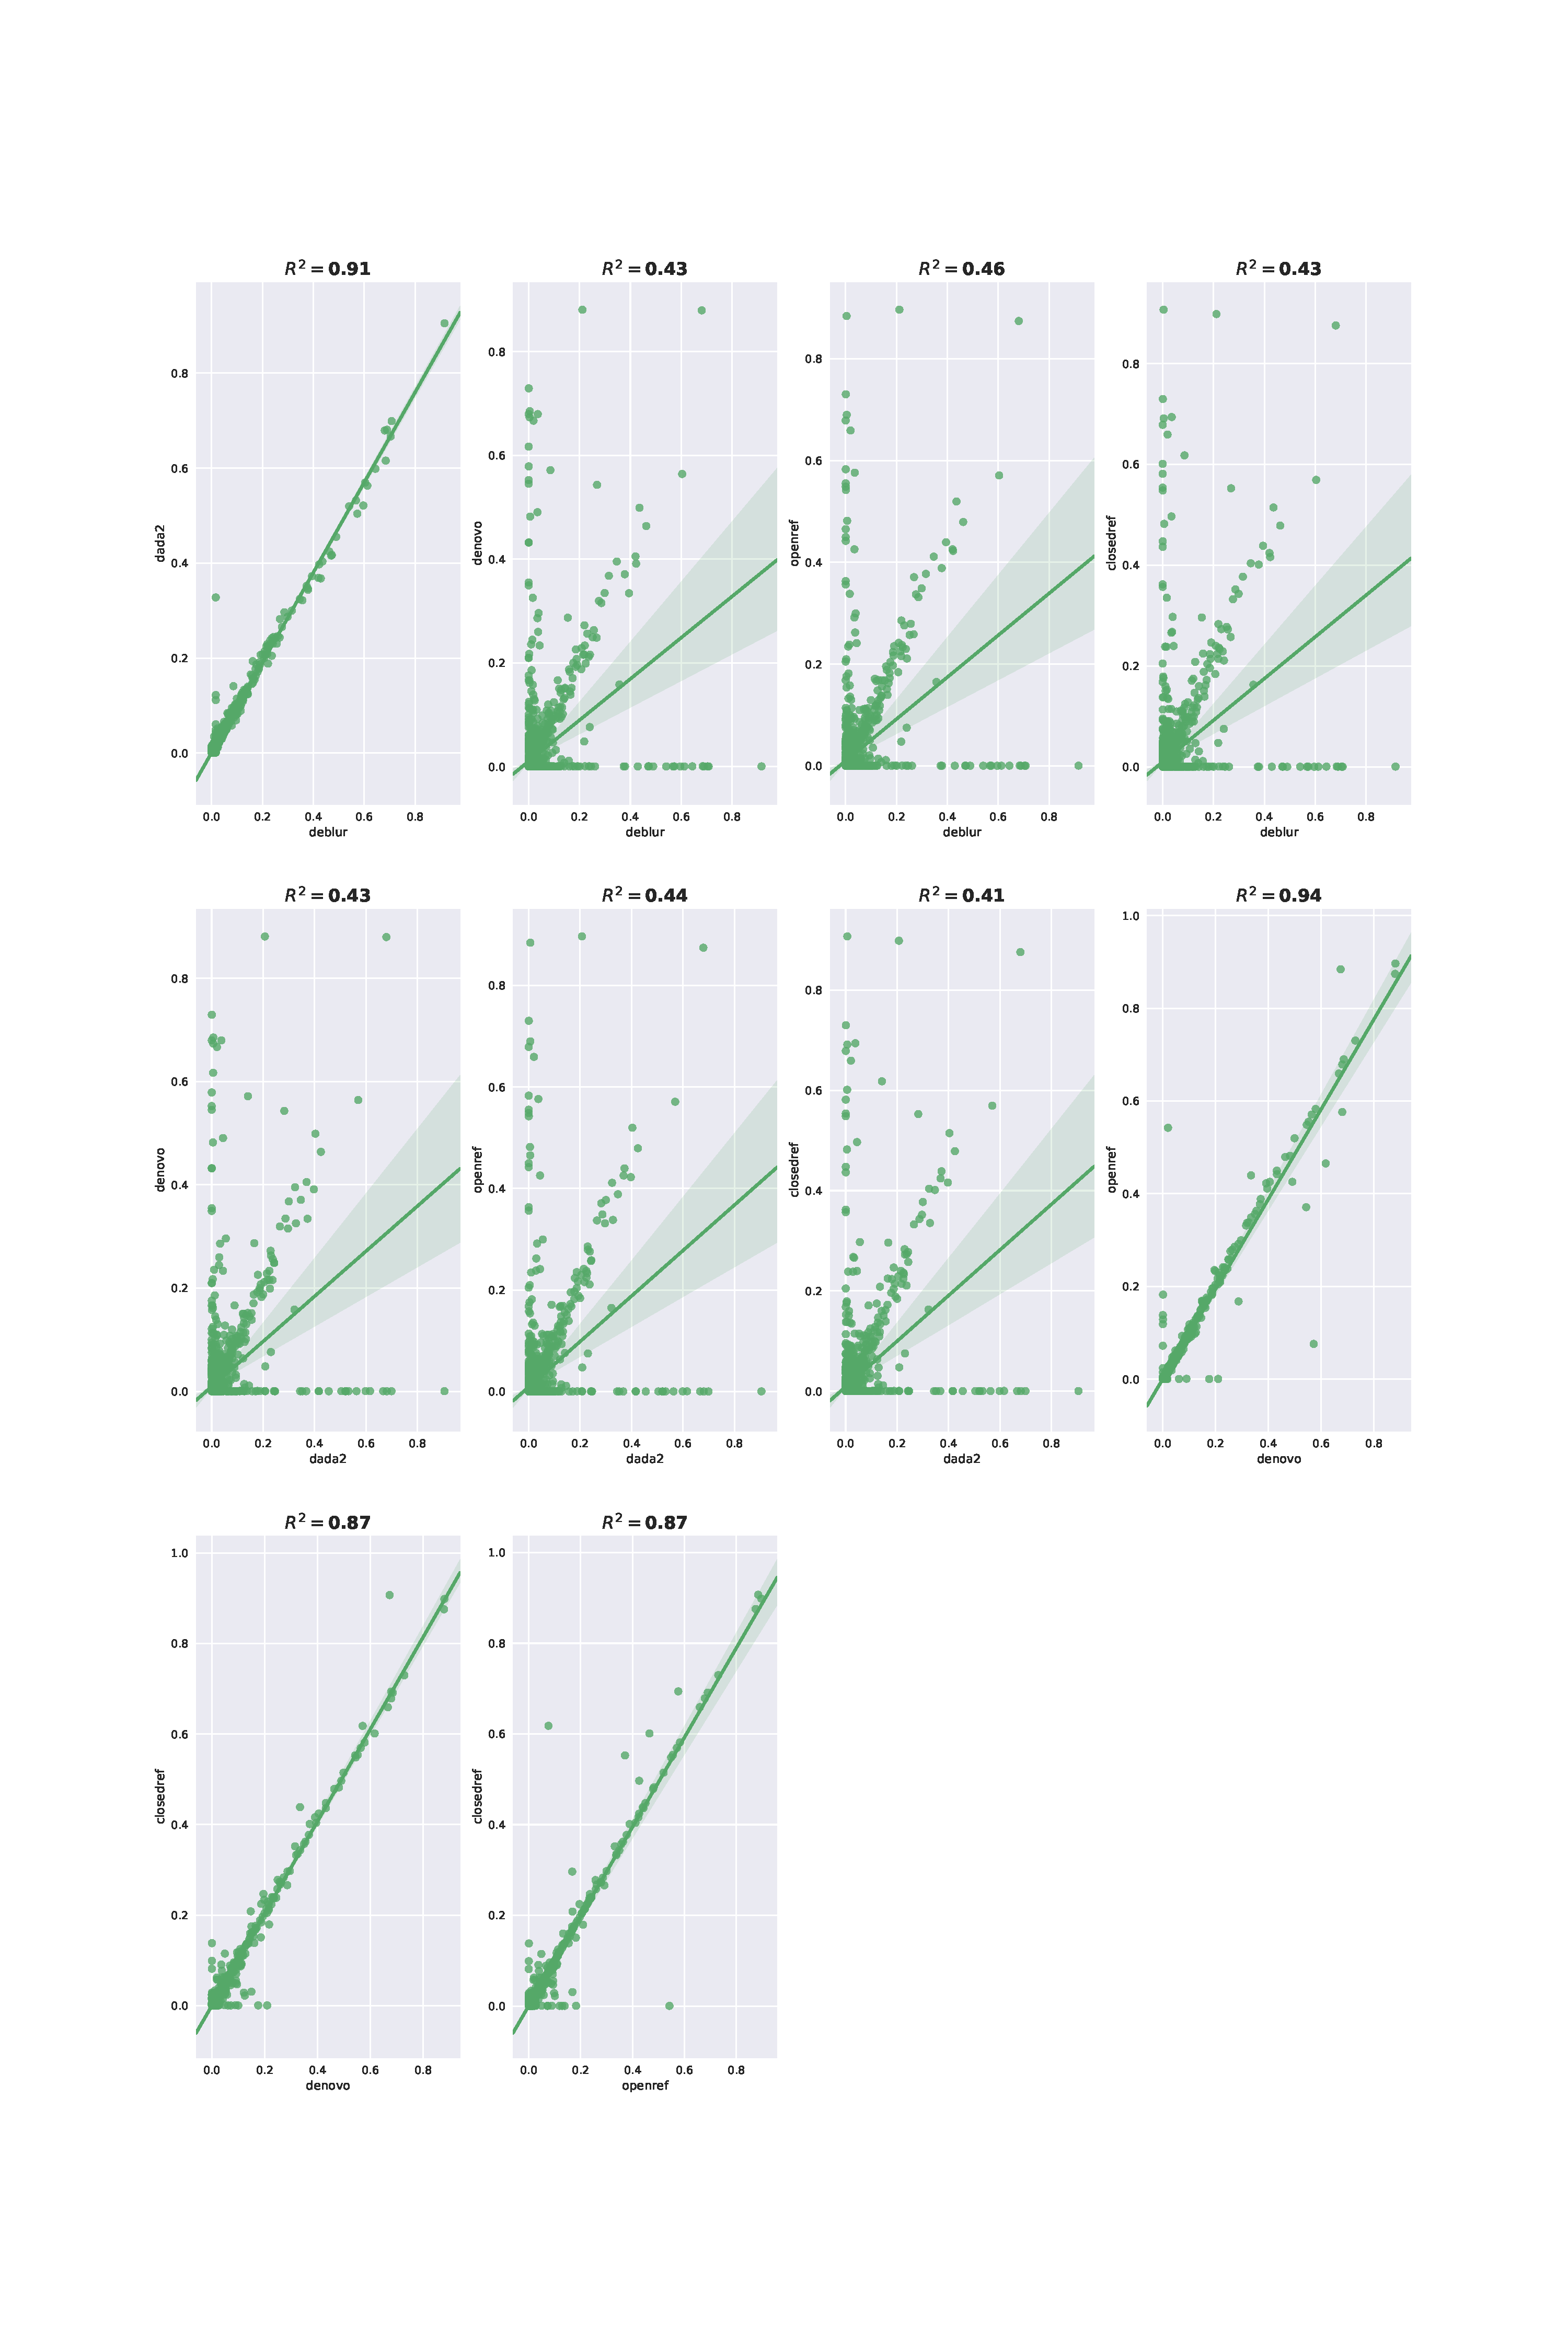
\includegraphics[width=0.9\linewidth]{pdf/all_denoise_reg.pdf}
%     \caption*{All pairwise correlations comparing the similarity between different denoising and clustering methods}
%     \label{fig:figureS4}
%   \end{figure}

  \begin{figure}[h]
    \centering
    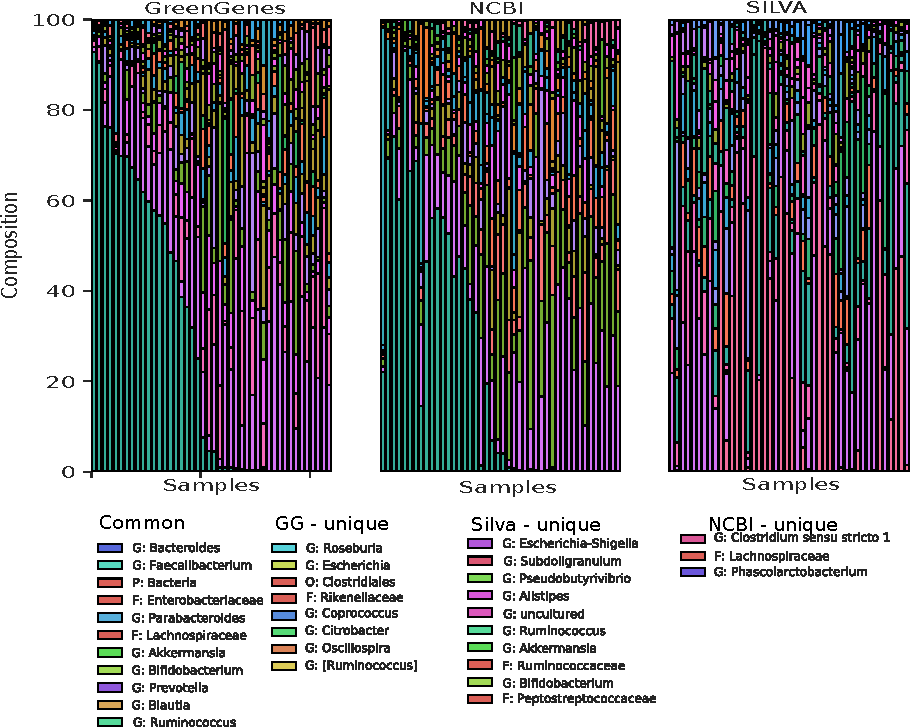
\includegraphics[width=\linewidth]{figureS4.pdf}
    \caption{
      \textbf{(A)} Taxonomy composition of the 20 most abundant genera predicted for the stool microbiome dataset generated using different taxonomy references databases: Greengenes, SILVA and NCBI.
      The legend shows the common and the unique genera among the taxonomy assignments.
  }
    \label{fig:figureS4}
  \end{figure}

  \begin{figure}[h]
    \centering
    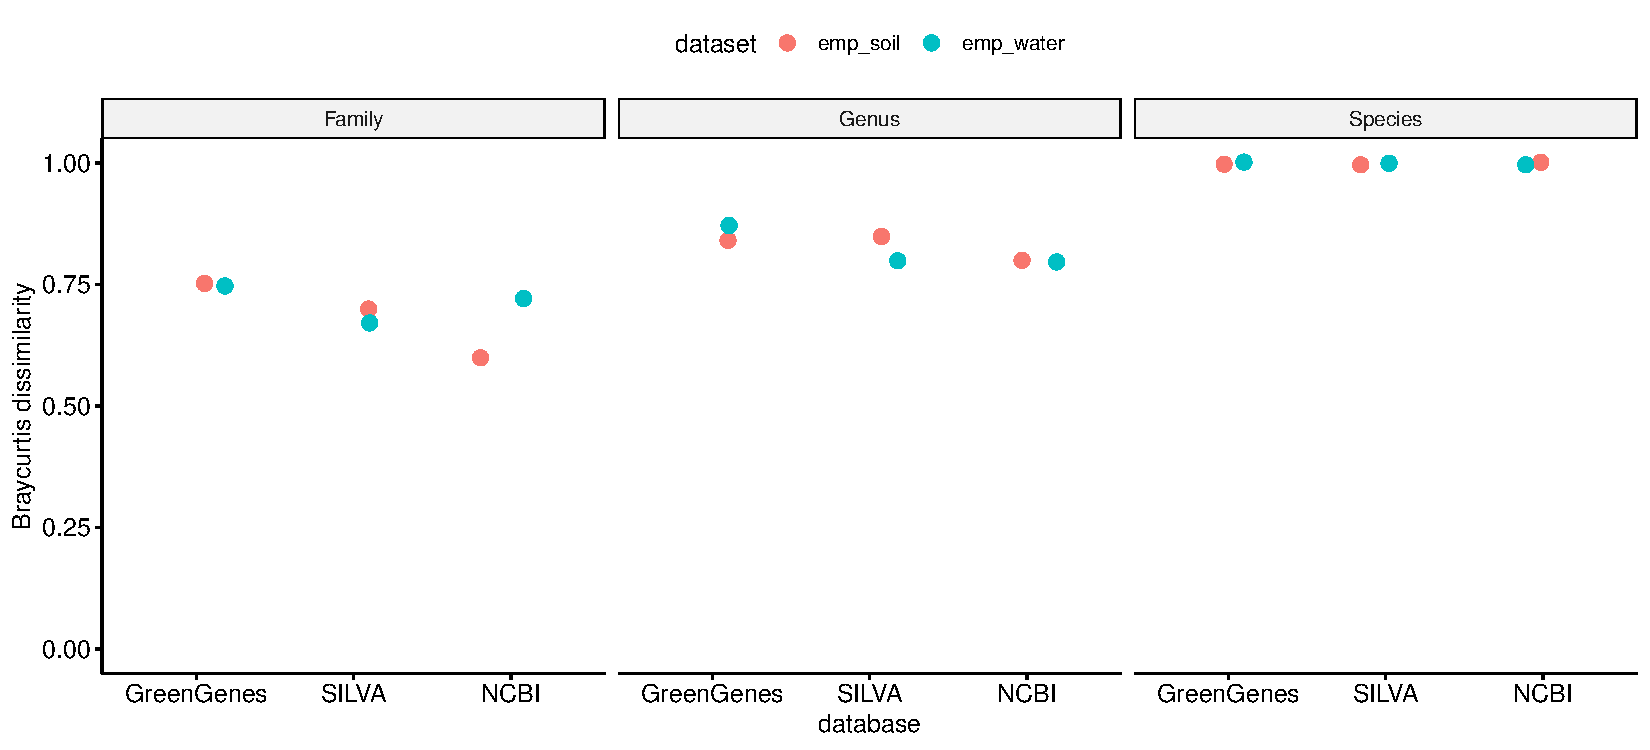
\includegraphics[width=\linewidth]{figureS5.pdf}
    \caption{
      The bray-curtis dissmilarity between the expected taxonomic composition and generated taxonomic composiion for the synthetic datasets.
  }
  \label{fig:figureS5}
  \end{figure}

%   \begin{figure}[h]
%     \centering
%     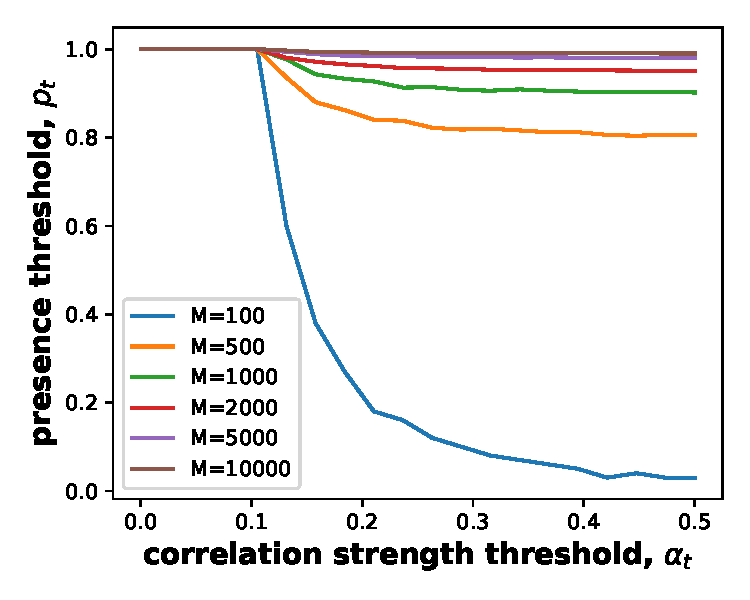
\includegraphics[width=\linewidth]{figureS6.pdf}
%     \caption{
%       Calculation of presence threshold that is applied on the OTU table in the OTU processing (OP) step of the pipeline.
%       This presence threhold $p_t$ is dependent on the number of samples in the dataset and the required correlation stength threshold.
%   }
%     \label{fig:figureS6}
%   \end{figure}

  \begin{figure}[h]
    \centering
    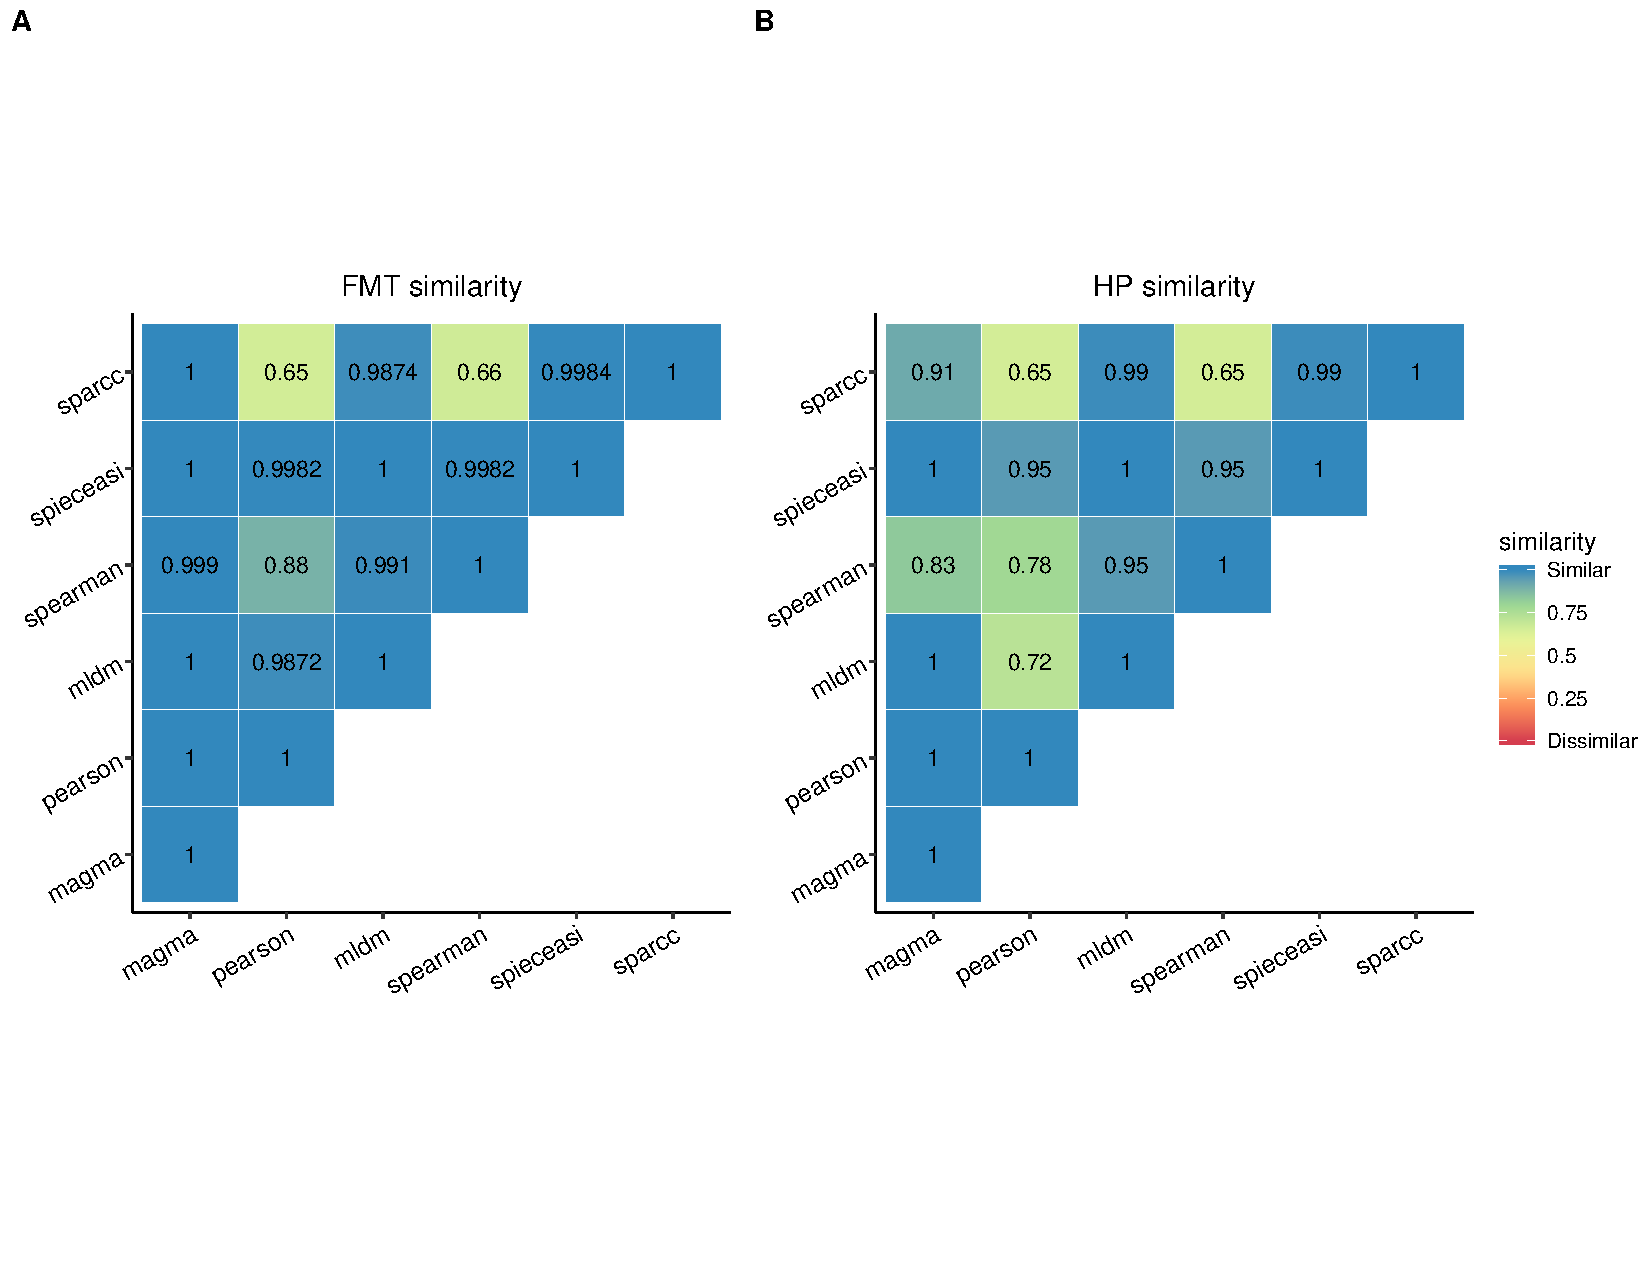
\includegraphics[width=\linewidth]{figureS8.pdf}
    \caption{
      The similarity between the networks generated using the different network inference algorithms for stool dataset (A) and the hard palate dataset (B).
      The similarity between the various methods was found to vary with the dataset used.
  }
    \label{fig:figureS8}
  \end{figure}

  \begin{figure}[h]
    \centering
    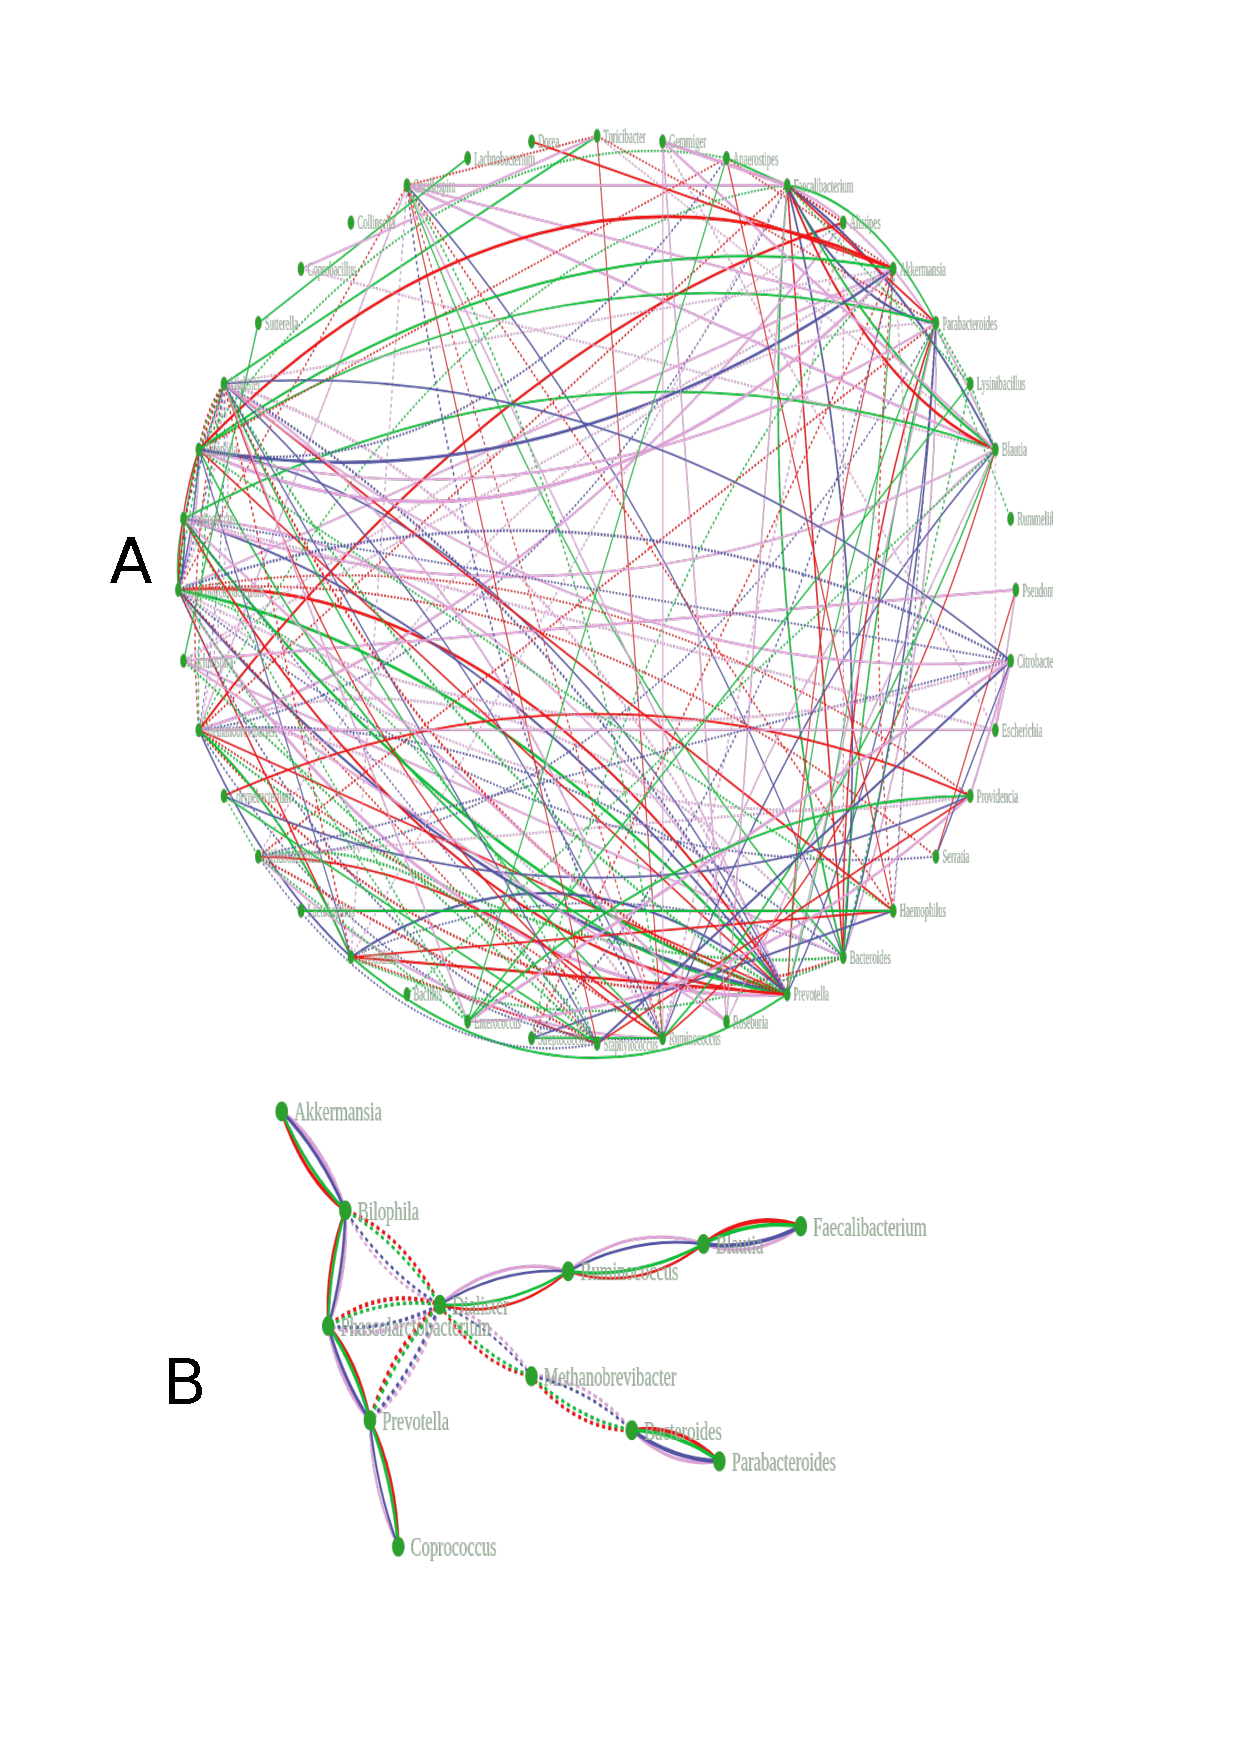
\includegraphics[width=0.8\linewidth]{pdf/denoise_network.pdf}
    \caption{A network showing union (A) and intersection (B) of networks generated using different denoising and clustering tools on the Stool dataset.}
    \label{fig:figureS5}
  \end{figure}
